%%
%% This is file `sample-sigconf.tex',
%% generated with the docstrip utility.
%%
%% The original source files were:
%%
%% samples.dtx  (with options: `sigconf')
%% 
%% IMPORTANT NOTICE:
%% 
%% For the copyright see the source file.
%% 
%% Any modified versions of this file must be renamed
%% with new filenames distinct from sample-sigconf.tex.
%% 
%% For distribution of the original source see the terms
%% for copying and modification in the file samples.dtx.
%% 
%% This generated file may be distributed as long as the
%% original source files, as listed above, are part of the
%% same distribution. (The sources need not necessarily be
%% in the same archive or directory.)
%%
%% The first command in your LaTeX source must be the \documentclass command.
\documentclass[sigconf, review]{acmart}
\usepackage{multirow}

%%
%% \BibTeX command to typeset BibTeX logo in the docs
\AtBeginDocument{%
  \providecommand\BibTeX{{%
    \normalfont B\kern-0.5em{\scshape i\kern-0.25em b}\kern-0.8em\TeX}}}


%% Rights management information.  This information is sent to you
%% when you complete the rights form.  These commands have SAMPLE
%% values in them; it is your responsibility as an author to replace
%% the commands and values with those provided to you when you
%% complete the rights form.
%\setcopyright{acmcopyright}
%\copyrightyear{2018}
%\acmYear{2018}
%\acmDOI{10.1145/1122445.1122456}

%% These commands are for a PROCEEDINGS abstract or paper.
%\acmConference[Woodstock '18]{Woodstock '18: ACM Symposium on Neural
%  Gaze Detection}{June 03--05, 2018}{Woodstock, NY}
%\acmBooktitle{Woodstock '18: ACM Symposium on Neural Gaze Detection,
%  June 03--05, 2018, Woodstock, NY}
%\acmPrice{15.00}
%\acmISBN{978-1-4503-XXXX-X/18/06}


%%
%% Submission ID.
%% Use this when submitting an article to a sponsored event. You'll
%% receive a unique submission ID from the organizers
%% of the event, and this ID should be used as the parameter to this command.
%%\acmSubmissionID{123-A56-BU3}

%%
%% The majority of ACM publications use numbered citations and
%% references.  The command \citestyle{authoryear} switches to the
%% "author year" style.
%%
%% If you are preparing content for an event
%% sponsored by ACM SIGGRAPH, you must use the "author year" style of
%% citations and references.
%% Uncommenting
%% the next command will enable that style.
%%\citestyle{acmauthoryear}

%\usepackage{libertine}

\usepackage{booktabs}
\usepackage{subfigure}
\usepackage{xspace}
%%\usepackage{amsmath}
\usepackage{epstopdf} 
\usepackage{algorithm}
\usepackage{url}
%%\usepackage{algorithmicx} 
\usepackage{algpseudocode}
%%\usepackage{color}
\usepackage{ulem}

\newcommand{\comments}[2]{{\bf[\textcolor{blue}{#1}: \textcolor{red}{#2}]}}

%\newcommand{\codecomment}[1] {\emph{\small{//#1}}}
\newcommand{\codecomment}[1] {\textit{\small{//#1}}}
\newcommand{\codelinecomment}[1]{\textit{\small{/* #1 */}}}

\newcommand{\codepink}[1]{\textcolor{magenta}{#1}}
\newcommand{\codeblue}[1]{\textcolor{blue}{#1}}

\newcommand{\green}[1]{\textcolor{black}{#1}}
\newcommand{\blue}[1]{\textcolor{blue}{#1}}
\newcommand{\red}[1]{\textcolor{red}{\sout{#1}}}
\newcommand{\pink}[1]{\textcolor{purple}{#1}}
\newcommand{\hlight}[1]{\textcolor{purple}{#1}}
\newcommand{\liuq}[1]{\comments{QLiu}{#1}}
\newcommand{\zfz}[1]{\comments{Fengzhe}{#1}}
\newcommand{\zwh}[1]{{\comments{Weihua}{#1}}}


\newcommand{\btree} {B+tree\xspace}
\newcommand{\txtree}{STM-based GPU \btree\xspace}
\newcommand{\base}{STM-based GPU B+tree\xspace}
\newcommand{\baseshort}{STM GB-tree\xspace}
\newcommand{\locktree}{lock-baed GB-tree\xspace}
\newcommand{\ucdavis}{lock-based GPU B-tree\xspace}
\newcommand{\ucdavisshort}{Lock GB-tree\xspace}


%\newcommand{\sys} {Rola-tree\xspace}
%\newcommand{\Sys} {Rola-tree\xspace}
\newcommand{\sys} {Eirene\xspace}
\newcommand{\Sys} {Eirene\xspace}

\newcommand{\trueconflicts}{key conflicts\xspace} %plural form
\newcommand{\trueconflictsCapital}{Key conflicts\xspace}
\newcommand{\falseconflicts}{structure conflicts\xspace}
\newcommand{\falseconflictsCapital}{Structure conflicts\xspace}

\newcommand{\trueconflict}{key conflict\xspace} % singular form
\newcommand{\falseconflict}{structure conflict\xspace}

%A,B,C,D represents the 4 column in overall performance. 5%update 95%search

%\newcommand{\speedupBtoA} {2.0} % for zipf 
%\newcommand{\speedupCtoA} {8.38} % for zipf 
%\newcommand{\speedupDtoA} {9.94} % for zipf 

\newcommand{\speedupBtoA} {1.3} % for uniform
\newcommand{\speedupCtoA} {5.9}	% for uniform
\newcommand{\speedupDtoA} {9.0}	% for uniform


\newcommand{\speedupLittleRatioCtoA} {5.15\xspace}
\newcommand{\speedupLittleRatioDtoA} {9.84\xspace}
\newcommand{\speedupBigRatioCtoA} {7.65\xspace}
\newcommand{\speedupBigRatioDtoA} {10.24\xspace}

\newcommand{\rangeFourTP}{603\xspace} % average throughput of different tree size
\newcommand{\rangeEightTP}{504\xspace}

\newcommand{\rangeFourUcdavis}{218\xspace}
\newcommand{\rangeEightUcdaivs}{173\xspace}
\newcommand{\rangeFourDtoU}{2.8}
\newcommand{\rangeEightDtoU}{2.9}


\newcommand{\tpNomerge}{838\xspace}
\newcommand{\tpC}{753\xspace}
\newcommand{\tpD}{1.11\xspace}			%average throughput of D
\newcommand{\tpDReadOnly}{1.33\xspace}	%All queries throughput
\newcommand{\mergeoptUnderline}{\uline{R}ecord-access merging\xspace}
\newcommand{\mergeopt}{record-access merging\xspace}
\newcommand{\mergeoptFirstCapital}{Record-access merging\xspace}
\newcommand{\mergeoptAllCapital}{Record-Access Merging\xspace}

\newcommand{\optimisticoptUnderline}{\uline{O}ptimistic write protection\xspace}
\newcommand{\optimisticopt}{optimistic write protection\xspace}
\newcommand{\optimisticoptFirstCapital}{Optimistic write protection\xspace}
\newcommand{\optimisticoptCapital}{Optimistic Write Protection\xspace}

\newcommand{\warpopt}{locality-aware warp reorganization\xspace}
\newcommand{\warpoptFirstCapital}{Locality-aware warp reorganization\xspace}
\newcommand{\warpoptCapital}{Locality-Aware Warp Reorganization\xspace}
\newcommand{\warpoptUnderline}{\uline{L}ocality-\uline{A}ware warp reorganization\xspace}

\newcommand{\optA}{\textit{TX \btree w merge}\xspace}
\newcommand{\optB}{\textit{TX \btree w merge+os}\xspace}
\newcommand{\optC}{\textit{TX \btree w merge+os+buf}\xspace}

\newcommand{\speedupToMasstree}{4.3}
\newcommand{\speedupToEuno}{2.7}
\newcommand{\HamoToTx}{36}

\newcommand{\speedupDtoU}{4.6}
\newcommand{\speedupCtoU}{3.0}

\newcommand{\Query}{\textit{Que\-ry}\xspace}
\newcommand{\query}{\textit{que\-ry}\xspace}
%\newcommand{\modify}{\textit{modify}\xspace}
\newcommand{\update}{\textit{up\-da\-te}\xspace}  % \- :  wrap line if need 
\newcommand{\del}{\textit{dele\-te}\xspace}
\newcommand{\rangequery}{\textit{range query}\xspace}
\newcommand{\rangequeries}{\textit{range queries}\xspace}
\newcommand{\Rangequery}{\textit{Range query}\xspace}
\newcommand{\Rangequeries}{\textit{Range queries}\xspace}
%\newcommand{\mixed}{\textit{get-put-delete-mixed}\xspace}
%\newcommand{\getkernel}{query kernel\xspace}
%\newcommand{\updatekernel}{update kernel}


%%
%% end of the preamble, start of the body of the document source.
\begin{document}

%%
%% The "title" command has an optional parameter,
%% allowing the author to define a "short title" to be used in page headers.
\title{Unified Virtual RDMA for Hybrid Virtual Environments}


%%
%% The "author" command and its associated commands are used to define
%% the authors and their affiliations.
%% Of note is the shared affiliation of the first two authors, and the
%% "authornote" and "authornotemark" commands
%% used to denote shared contribution to the research.
\iffalse 
\author{Ben Trovato}
\authornote{Both authors contributed equally to this research.}
\email{trovato@corporation.com}
\orcid{1234-5678-9012}
\author{G.K.M. Tobin}
\authornotemark[1]
\email{webmaster@marysville-ohio.com}
\affiliation{%
  \institution{Institute for Clarity in Documentation}
  \streetaddress{P.O. Box 1212}
  \city{Dublin}
  \state{Ohio}
  \country{USA}
  \postcode{43017-6221}
}
\fi


%%
%% By default, the full list of authors will be used in the page
%% headers. Often, this list is too long, and will overlap
%% other information printed in the page headers. This command allows
%% the author to define a more concise list
%% of authors' names for this purpose.
\renewcommand{\shortauthors}{}

%%
%% The abstract is a short summary of the work to be presented in the
%% article.

\begin{abstract}
Supercomputing is important in most data-driven fileds for its extrem high-performance, such as such as artificial intelligence and large-scale data processing. As the developement of cloud, supercomputing is also in virtual machines or containers for effiecncy and elasticity. Today, hybrid virtual enviroments is a trend in most datacenters because of combined advatanges and historic reasons. RDMA is neccesay in supercomputing for its high network performance. However, existing RDMA virtualization solutions lack centralized virtualization layer and general interfaces for hybrid virtual environments. To solve this problem, we present uniRDMA, a generic RDMA software virtualization framework that consists of single virtual layer and general uniVerbs interfaces. The centralized user space virtual layer constructs multiple isolated vRNICs(virtual RDMA NICs) with the help of hardware virtualization technology and realizes a unified virtual RDMA network. To realize both generality and high-performance, uniVerbs interfaces use shared memory as I/O approach for RDMA applications and map RDMA resources to vRNIC. In our evaluation based on uniRDMA prototype, the performance and scalability of uniRDMA is close to bare-metal RDMA in virtual machines, containers and hybrid cloud environments.
\end{abstract}



%%
%% The code below is generated by the tool at http://dl.acm.org/ccs.cfm.
%% Please copy and paste the code instead of the example below.
%%

%\begin{CCSXML}
%<ccs2012>
% <concept>
%  <concept_id>10010520.10010553.10010562</concept_id>
%  <concept_desc>Computer systems organization~Embedded systems</concept_desc>
%  <concept_significance>500</concept_significance>
% </concept>
% <concept>
%  <concept_id>10010520.10010575.10010755</concept_id>
%  <concept_desc>Computer systems organization~Redundancy</concept_desc>
%  <concept_significance>300</concept_significance>
% </concept>
% <concept>
%  <concept_id>10010520.10010553.10010554</concept_id>
%  <concept_desc>Computer systems organization~Robotics</concept_desc>
%  <concept_significance>100</concept_significance>
% </concept>
% <concept>
%  <concept_id>10003033.10003083.10003095</concept_id>
%  <concept_desc>Networks~Network reliability</concept_desc>
%  <concept_significance>100</concept_significance>
% </concept>
%</ccs2012>
%\end{CCSXML}
%
%\ccsdesc[500]{Computer systems organization~Embedded systems}
%\ccsdesc[300]{Computer systems organization~Redundancy}
%\ccsdesc{Computer systems organization~Robotics}
%\ccsdesc[100]{Networks~Network reliability}

%%
%% Keywords. The author(s) should pick words that accurately describe
%% the work being presented. Separate the keywords with commas.
\keywords{RDMA, Virtulization, Hybrid Virtual Environment}



%%
%% This command processes the author and affiliation and title
%% information and builds the first part of the formatted document.
\maketitle

\section{Introduction}
RDMA(remote direct memory access), is a new type of high-performance network technology. RDMA is currently widely used in artificial intelligence, data processing, and high-performance computing. For examples, TensorFlow, Spark, and Hadoop [21] all have supported RDMA. With hardware protocol stack and zero copy technologies, RNICs(physical RDMA network cards) can bypass the kernel to read/write remote memory data according to the work requests of applications, without the participation of remote CPU. Therefore, RDMA has high throughput, low latency and low CPU load.

The core technology of cloud computing is virtualization, mainly including container and virtual machine. The container is a lightweight isolated runtime environment, does not need device emulation, and has low performance loss. The virtual machine has strong isolation and is more secure, but the performance loss is large. Both virtual machines and containers have been widely used, and the trend has become the unified deployment and management for hybrid virtual environments. For example, VMware's virtualization platform vSphere and ReadHat's container cloud platform OpenShift, both clearly support the unified deployment and management of virtual machines and containers in the latest version.

RDMA virtualization is necessary for cloud applications to exploit RDMA. RDMA virtualization not only needs to maintain high performance and manageability, but also have generality for hybrid virtual environments. Therefore, our RDMA virtualization goals are as follows:

\begin{itemize}
\item {\verb|Generality|}: To form unified RDMA virtualization, single centralized virtual layer should be set up, which is provided to virtual machines and containers with general interfaces.
\item {\verb|High performance|}: Virtual RDMA should be close to native RDMA in terms of throughput, latency, and CPU load. Meanwhile it should be suit for large-scale virtual cluster.
\item {\verb|High manageability|}: In RDMA virtualization, container and virtual machine characteristics should be maintained to realize portability, isolation and network management.
\end{itemize}

RDMA has different hardware characteristics and working mechanisms compared to traditional network. Therefore, RDMA virtualization is different from traditional network virtualization. Current RDMA virtualization work mainly includes hardware virtualization and software virtualization. However, none of the existing solutions can meet all above goals.

The representative of hardware virtualization is SR-IOV. Its virtual layer is located in the hardware. Although the isolation and high performance are maintained,  SR-IOV lacks portability and other manageability without software virtual layer. In software virtualization, existing solutions treat virtual machines and containers differently. For containers, FreeFlowl~\cite{kim2019freeflow} forwards all RDMA commands to the virtual layer, and that is ineffective because of losing RDMA's kernel by-pass. For virtual machines, HyV avoids forwarding overhead by mapping RDMA resources, but lacks the management of virtual RDMA networks; although MasQ makes up for this problem, its virtual layer is located in kernel space. Extending MasQ to the container environment will lose lightweight  management in user space for containers.

We proposes an unified RDMA virtualization framework for both containers and virtual machines, namely uniRDMA, which achieves high performance and high manageability. UniRDMA is mainly composed of single centralized uniRDMA virtual layer and general uniVerbs interfaces. All managements are concentrated in the user space virtual layer; the UniVerbs interface is general to the RDMA applications in virtual machines or containers.

There are mainly two challenges in the design of uniRDMA: First, virtual machines and containers are essentially different virtualization technologies. Virtual machines are under the management of hypervisor in kernel space, containers are isolted runtime mainly about user space. It is a challenge to build a centralized virtual layer for both containers and virtual machines; second, mapping all RDMA resources is the key idea to achive high performance. However, the existing solutions only implement the mapping operation in the same process for virtual machine. In this paper, the virtual layer belongs to another host process. So, it is also another challenge to map all RDMA resources.

To address the first challenge, uniRDMA separates the control and use of RDMA resources in virtulization, builds multiple vRNICs in single unified user space virtualization layer. Each vRNIC encapsulates virtual RDMA resources, and isolates with others by hardware virtualization. Moreover, through a common file-based shared memory queue, each vRNIC has a general interface for virtual machines and containers. For the second challenge,  at first, virtual RDMA resources in vRNICs are mapped to physical RNICs, and then shared memory are used to ensure RDMA resources in applications are mapped to vRNICs in the virtual layer.

We implements the prototype of uniRDMA and evaluate uniRDMA against with hardware virtualization, software virtualization FreeFlow, and native RDMA in different benchmarks, such as throughput, latency, scalability, and real-word applications. From the result, uniRDMA's performance is close to native RDMA in both virtual machine and container environments, and is significantly better than FreeFlow. The throughput can reach up to 6 times that of FreeFlow, and the latency can reach down to 40\% of FreeFlow.uniRDMA also has high scalability and adapts to real-world RDMA applications in hybrid cloud environments.

The main contributions in this paper are as follows:

(1)Unified RDMA virtulization in hybrid virtual environments is firstly proposed in this paper and uniRDMA is general RDMA virtualization framework,  while maintaining high performance and high manageability.

(2)uniRDMA are evaluated and the results proved that uniRDMA maintains high performance close to native RDMA.


\section{RDMA Background} \label{background}
RDMA infrastructure is built for distributed applications that require high-performance and low latency network communications. It uses a zero copy approach to deliver data between servers. With RDMA, applications can read and write memory of a remote machine, without the participation of CPU and OS kernel on both sides.

\begin{figure}[!ht]
	\centering
	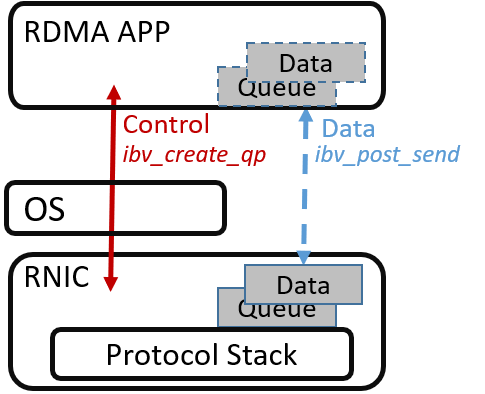
\includegraphics[width=0.8\linewidth]{images/rdma-feat.png}
	\caption{Native RDMA Architecture: the control path and data path are separated}
	\label{fig:rdma-feat}
\end{figure}

RDMA can be implemented in different ways, for example, InfiniBand~\cite{infiniband}, Roce~\cite{roce}, and iWARP~\cite{iwarp}.
OpenFabrics Enterprise Distribution (OFED \cite{ofed}) is a widely used RDMA software stack that builds an abstraction layer to hide the differences of underneath drivers and hardware.
OFED stack consists of the user-space part and the kernel-space part.
As shown in Figure~\ref{fig:rdma-feat}, in user-space, RDMA applications use Verbs APIs~\cite{verbs} to send and receive data. It is similar to socket layer for traditional network applications. On the control path, Verbs provides APIs like ibv\_create\_qp and ibv\_reg\_mr. On the data path, Verbs provides APIs like ibv\_post\_send and ibv\_post\_recv. On the control path, the Verbs library forwards requests to OFED core in OS kernel. Device specific drivers that control the RDMA hardware are registered in OFED core. On the data path, the OS kernel is bypassed. So the Verbs library calls device specific user level library to send and receive data.

In the workflow of RDMA, the control path and the data path are separated. As shown in Figure~\ref{fig:rdma-feat}, on the control path, the application explicitly creates QP~(Queue Pair), CQ~(Completed Queue), registers MR~(Memory Region) and other RDMA metadata, and caches the metadata to RNIC, such as queue ID, MR key and page tables. On the data path, the application can write to the DoorBell register to notify RNIC of a new request. RNIC will read the request in the QP, read/write the contents of the local/remote MR, and put the completion notifications into the CQ. The application can poll the CQ to get the notifications. The housekeeping work is done on the control path that involves the OS kernel. The performance critical data transmission work on the data path totally bypasses the OS kernel.
\section{Overview}
The architecture of uniRDMA is shown in Figure~\ref{fig:framework-overview}. uniRDMA mainly consists of vRNIC, which is a para-virtualization device for guest, and the management layer(虚拟层暂定为管理层). Besides, some modifications are made to RDMA user library and device specific drivers for cooperating with uniRDMA.

(1) vRNIC frontend and backend: vRNIC frontend is as the device driver of hosts' backend. It cooperates with modified verbs and device-specific libraries and forwards serial commands to backend. In specific, the frontend is in kernel for VMs. vRNIC backend is as virtual device in host user space. It execute received commands. To achieve high performance, the control path and data path are separate in vRNICs. For data path, vRNIC frontend does not forwards RDMA commands, and directly use the mapped RDMA resources (e.g. QPs or MRs). The resources are mapped to backend by shared memory.

(2) Management Layer: To make a centralized management, a management center connect with each host's uniRDMA backend. The management mainly includes vRNIC device management and network management. For device management, the layer coordinates the hardware resources (e.g. VFs in SR-IOV) to achieve the hardware-support functions effectively, e.g. performance isolation. For network management, the layer can construct a virtual RDMA network by software methods, including configuring each vRNIC address, defining routing rules and maintaining the mapping for vRNIC connections. (包含设备管理和网络管理两个部分,设备管理主要是协调硬件虚拟化VF资源,网络管理是纯软件实现,包括配置vRNIC地址和路由规则等)

Besides, to support transparency for applications in guest, we modified the verbs library and hardware-specific libraries in guest. After modification, the RDMA commands can be forwarded to vRNIC frontends. Also, the memory of RDMA resources (e.g. QPs) can be backend with our shared memory. (必须修改设备相关库,RDMA QP资源的内存才能够用我们的共享内存去支持)

\begin{figure}[!ht]
	\centering
	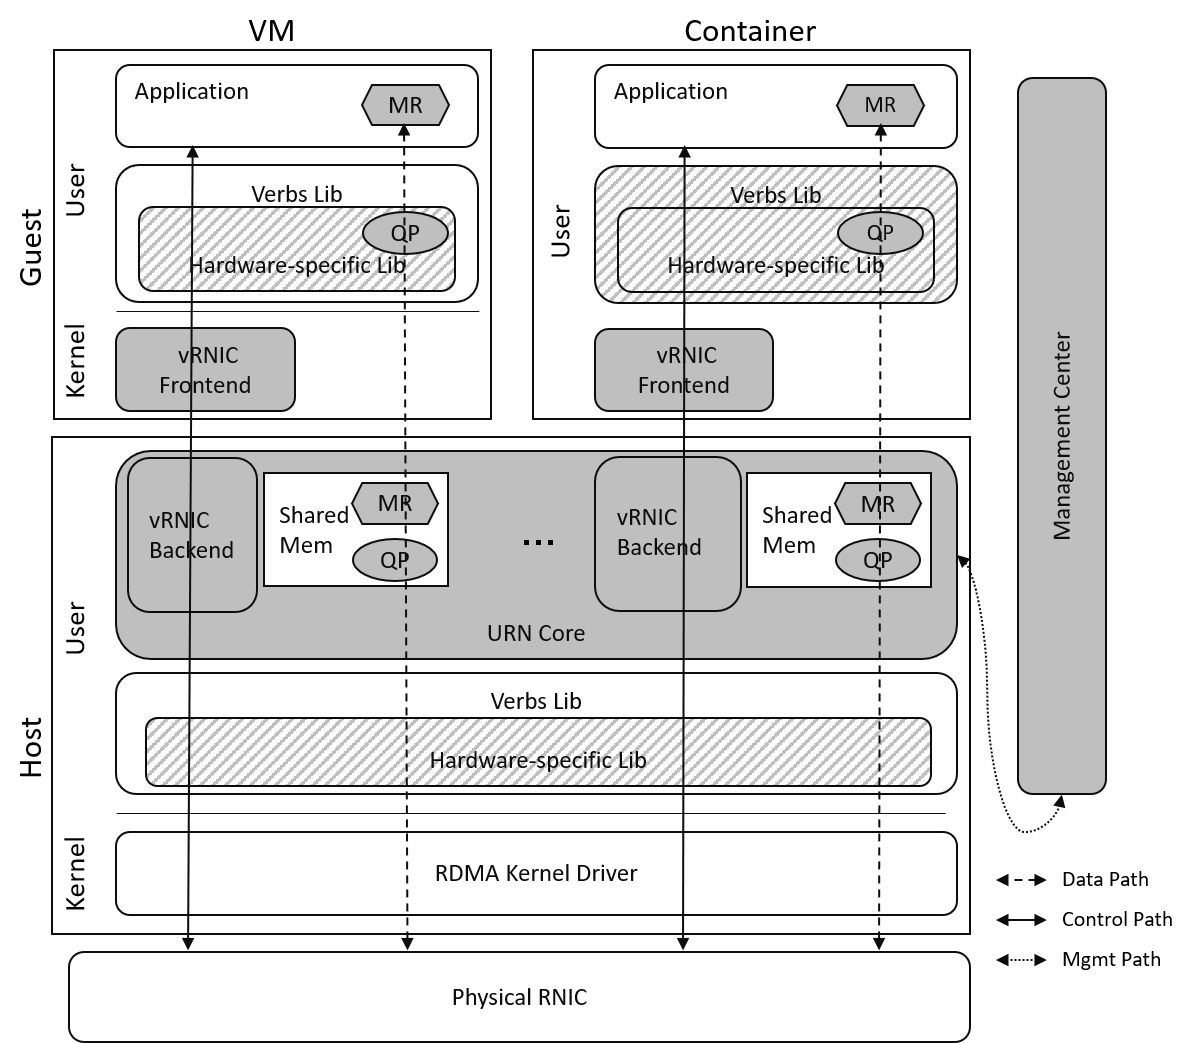
\includegraphics[width=1\linewidth]{images/framework-overview.png}
	\caption{uniRDMA Framework Overview}
	\label{fig:framework-overview}
\end{figure}
\section{vRNIC Design}
To achieve unified RDMA virtualization, we design vRNICs, which is software virtualization with complete RDMA attributes (e.g. QPs). Both conatiners and VMs can use vRNICs through unified drivers. In this section, we firstlly introduce vRNIC virtualization and its driver. Then, optimizations for performance are introduced.

\subsection{vRNIC Virtualization}
To make vRNIC flexible and hardware-independent, we construt each vRNIC in host by software methods. Besides, software methods are more scalable and isolated for VMs or containers.

Moreover, both kernel-space and user-space are feasible to construct vRNICs in host. Compared to kernel-space, there are multiple advantages for vRNICs in user-space, such as minimal attack surface, flexible management and independent on RDMA kernel drivers. Thus, we choose the user-space for vRNIC virtualization.

\subsubsection{Static Attributes} ~\\
In summary, RNIC has two kinds of hardware properties, namely static property and dynamic property: Static attributes mean unchanged and unrecorded attributes in physical RNIC. For example, the device name and resource handle are both static for RNIC. Compared, dynamic attributes means they should be recorded into or generated from hardware exiplictly. For example, QP is dynamic beacause it should to be reflected in RNIC.

For static attributes, we directly use virtual names for them. For example, the device name of vRNIC is virtual. Besides, the address of vRNIC is also virtual. There are two main advantages for these: first, virtual information hids the real hardware informations for clouds' user; second, virtual information, especially virtual address is basic to construct a virtual network. 
\subsubsection{Dynamic Attributes} ~\\
However, for dynamic attributes, the hardware cannot regconize virtual informations. Thus, we need map the so-called virtual dynamic attributes to physical RNIC to make them effective. For example, when application calls post\_send, the vRNICs can drive physical RNIC to transport the corresponding data. Thus, in our design, the vRNIC is flexible for management. 

Fortunately, all RDMA resources information in RNIC are only changed in control path and maintained in data path. So, we can map the virtual RDMA resources to RNIC only in control path, such as QP and Doorbell,  and do not need introduce any operations in data path. Mapped RDMA resources are directly used and RNIC is notified by mapped virtual DoorBell in vRNIC. As a result, vRNIC are still with DMA zero-copy, hardware protocol stack processing and other high-performance capability in data path. Therefore, we put each vRNIC with a map unit. As Figure~\ref{fig:map-unit} shows, it maps or unmaps virtual RDMA resources from vRNIC to RNIC in control path:-


\begin{figure}[!ht]
	\centering
	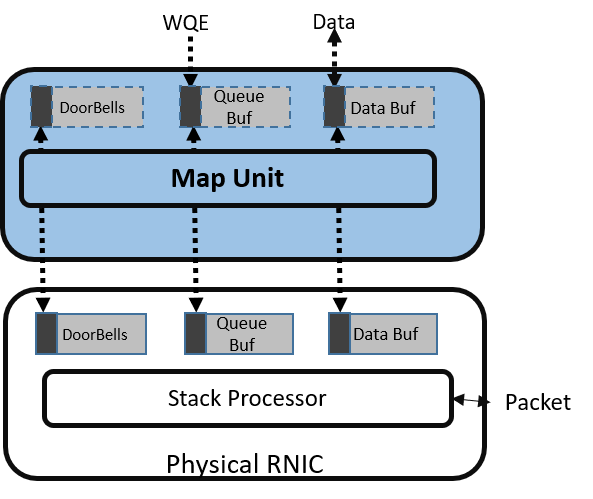
\includegraphics[width=0.9\linewidth]{images/map-unit}
	\caption{Map Unit in vRNIC}
	\label{fig:map-unit}
\end{figure}

For RDMA resources (e.g. QPs, CQs): Taking QP as an example, regularly, vRNIC record virtual RDMA resources information when the virtual QP instance are created. However, virtual QP are still not generated-associated with the RNIC. To make the mapping, the map unit will create corresponding real QP instance in RNIC based on the information of virtual QP instances, such as the same memory address information and the same device id. Equivalently, the virtual QP information are recognized in RNIC, such as QP number and QP state, and can be one-to-one synchronous with RNIC’s physical instance by lots of similar map operations in control path. All operations can be completed by calling the Verbs interface of RNIC in user space. After the mapping is completed, the work requests in the vRNIC virtual QP can be zero-copied into the RNIC. Also, data in registered memory of vRNIC can also be zero-copied to RNIC in the same way. 

For DoorBells: It needs to be mapped to the hardware doorbell in the physical NIC device space, so that vRNIC can notify the RNIC hardware processors. In vRNIC, the mapping unit will map the virtual address of the virtual doorbell to the hardware doorbell address of the corresponding physical NIC device space through a system call. As shown in Figure~\ref{fig:map-unit}, after the mapping is completed, the write operation to the vRNIC virtual doorbell is equivalent to performing the doorbell notification to the RNIC.

Map unit is the key for vRNICs' performance. Note that all mapping relationships are all one-to-one, therefore, the correctness and isolation of resources in different RDMA context are guaranteed. Meanwhile, because the mapping operation is only executed in control path, the overhead is one-off compared to data commands. For the data path, vRNICs can directly utilize the hardware processing capability of RNIC, such as DMA zero-copy and hardware protocol stack processing.

\subsection{Unified vRNIC Driver}
vRNIC is virtual device with complete RDMA attributes. However, vRNICs are still independent software in host user space. Thus, for VMs and containers, the driver (or library in containers) for vRNICs should be designed. Unification is necessrary for vRNIC driver, beacause it hides the difference of applications' environments and makes the centralized management (e.g. the virtual layer in later section) easier.

For containers, vRNICs can be directly provided to RDMA applications in containers with some modification in containers' verbs library. However, vRNICs  and VMs' application are isolated with the hypervisor and guest OS. vRNICs needs to be recongnized by VMs' hypervisor and then provided by guest OS. Thus, the I/O virtualization shoulde be used to extend each vRNIC for VMs. Then, specific driver for vRNICs installed in guest OS. 

However, the main challenge of above is how to make vRNICs unified to all RDMA applications. Thus, the comminucation between vRNIC to VMs or containers must be consistent. To make vRNICs communication consistent, we design a unified protocal from vRNIC to VMs' hypervisor or containers' applications. Note that both containers' applications and VMs are processes for host. Thus, I/O channel between vRNIC and VM is shared memory with specific protocal, e.g. vhost-user. And that is nature to containers' applications. Besides, the notification is used in event descriptor.

The goal of the device driver is to support I/O process inside each guest. As shown in in Figure~\ref{fig:vrnic-driver},  the commands of RDMA application be forwarded into the memory-shared queue, and trigger events to notify the vRNIC to process them; similarly, the device driver receives interrupt notifications and reads the result from vRNIC. In short, the device driver can be implemented by a lightweight kernel module.

\begin{figure}[!ht]
\centering
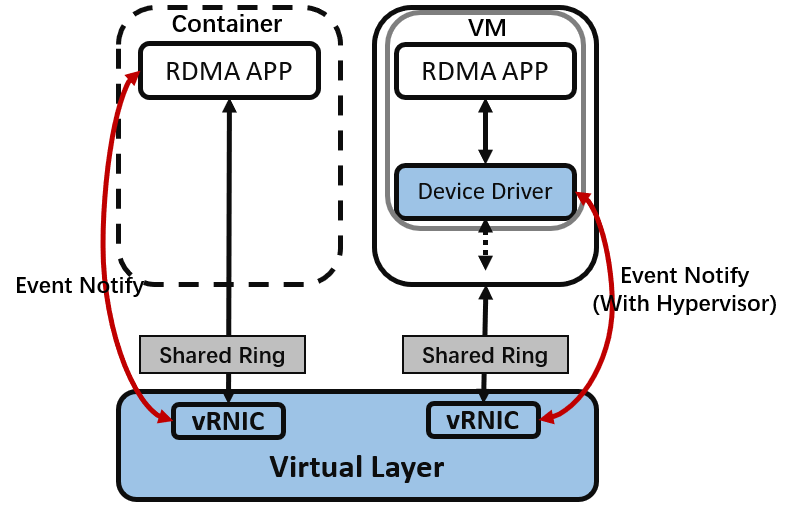
\includegraphics[width=1.0\linewidth]{images/interface-general}
\caption{Unified vRNIC Driver}
\label{fig:vrnic-driver}
\end{figure}

	
\subsection{Performance Optimization}
Trough vRNIC driver, all commands of RDMA applications can be excuted in vRNICs. However, in data path of vRNIC, there is still data-copy. Also, the data commands are forwarded to vRNIC for execution. These brings the data-copy or context-switch latency for RDMA applications. 

To address above performance problems, we map RDMA resources between vRNICs and appications. However, there are two different RDMA resources for vRNICs: resources in host physical memory (such as QPs, MRs), resources in physhical RNIC (e.g. DoorBell registers). 

(1) For QPs or MRs: The fact of zero-copy is that both processes have common available physical memory pages. Same as native RDMA, the zero-copy contents are including the RDMA work request in QPs and data in MRs. 
Similar as the above I/O channels, we use shared memory to map applications' memroy to vRNICs' RDMA resources (e.g. QPs and MRs). And this mapping is feasible for both VMs and containers.

\begin{figure}[!ht]
	\centering
	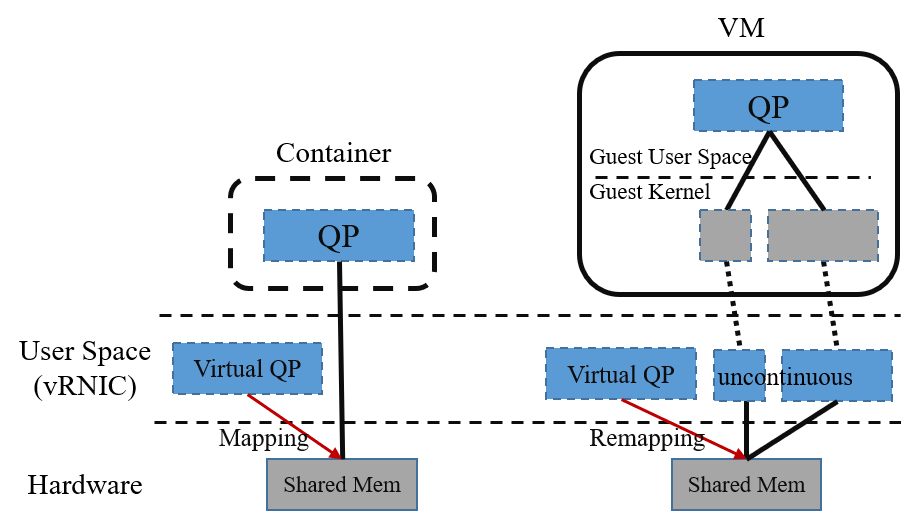
\includegraphics[width=1.0\linewidth]{images/zero-copy}
	\caption{Mapping QP to vRNIC}
	\label{fig:zero-copy}
\end{figure}

However, in the virtual machine, due to the memory management mechanism of guest operating system, the virtual machine's physical memory of the RDMA resource may be not continuous, and the mapped memory area in vRNIC is not continuous like Figure~\ref{fig:zero-copy}. So, vRNIC cannot map the virtual memory area as a virtual RDMA resource to RNIC. To solve this problem, the virtual memory remapping mechanism in user space is used. It remaps the discontinuous RDMA resource virtual memory area in vRNIC to the a block of continuous virtual memory, and the sequence of mapped physical memory page must be unchanged.

(2) For doorbells: Pressing the doorbell is necessary in RDMA data path to drive RNIC. In vRNIC, the doorbell that is mapped to physical RNIC, still need to be mapped to RDMA application to meet bypassing. Otherwise, the pressing command needs be forward to vRNIC and that’s imports apparent latency in data path.

However, the RDMA application and the vRNIC belong to two different processes on the host, and they have isolated virtual address spaces. At the same time, the doorbell register is in the device address space and cannot be mapped by shared memory. The key to solving this problem is that the process of RDMA application needs to know the physical address of the doorbell register.

\begin{figure}[!ht]
	\centering
	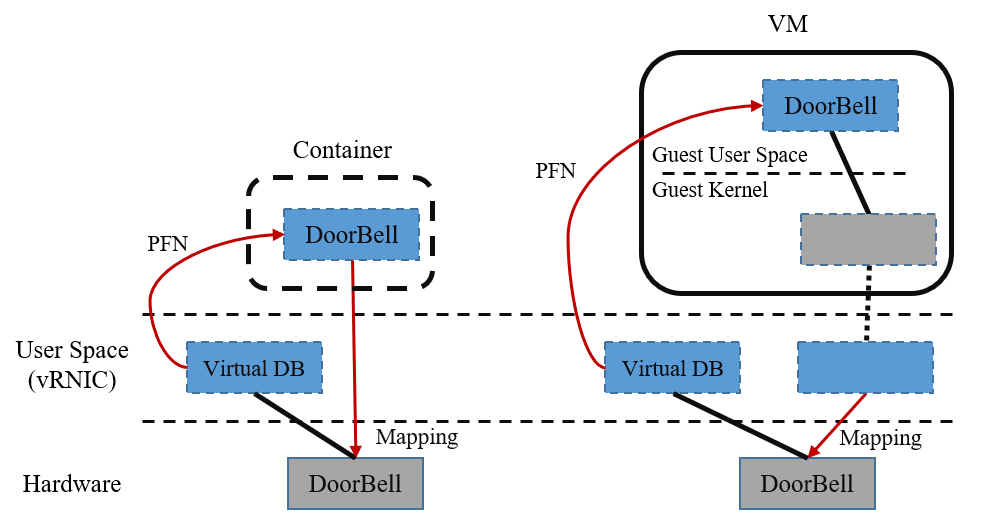
\includegraphics[width=1.0\linewidth]{images/by-pass}
	\caption{Mapping DB from vRNIC}
	\label{fig:by-pass}
\end{figure}

Therefore, when an RDMA application creates a RDMA context, as shown in Figure~\ref{fig:by-pass}, it sends a request to the vRNIC at first. Under the supervision of virtual layer, vRNIC forwarded to application with the corresponding physical address of the doorbell, commonly the physical page number. After that, the application maps its doorbell virtual address to the physical page in its own process, that needs the host kernel and hypervisor if the application in virtual machines.


\section{Management Design}
Managiability of virtualization is important for clouds. To manage vRNICs centrally, we design a virtual layer. The works of virtual layer are including vRNIC instantiation, vRNIC mapping to RNIC. Besides, virtual layer manages the virtual network for VMs or containers, such as configuring virtual vRNIC address, routing rules or more management in clouds.

\subsection{vRNIC Device Management}
Each vRNIC is instantiated in the virtual layer. We found that another difference for VMs and containers: VM is a unstopped process for host onece it boosts, even though RDMA applications in VM is not running; container's RDMA application is a regular process for host. Thus, we make static instantiation for VM's vRNIC before VM boosts, and make dynamic instantiation when the verbs library are loaded in container's application. In contrast, we destroy the vRNIC instance when VM stoping or container's application exiting. Besides saving system resources, another advantage of this is to avoid contend and assure corrects for multipe applications in one container. Note the contend for mutiple applications in one VM are solved with guest OS and our kernel vRNIC driver. The overhead of instantiation is one-time for VMs or containers' applications.

The virtual layer should manage the mapping from vRNIC to RNIC. To achive performance isolation, we utilize the SR-IOV, which virtualize multiple isolated VFs (different hardware interfaces) in one physical RNIC. The virtual layer maps vRNICs to VFs respectively. 

However, we note that VF resources of SR-IOV are limited, for example, only 126 VFs are supported in Mellanox ConnectX-3 at most~\cite{ofed-manual}. Therefore, the existing VFs need to be managed and coordinated in a unified to meet many vRNICs.

\begin{figure}[!ht]
	\centering
	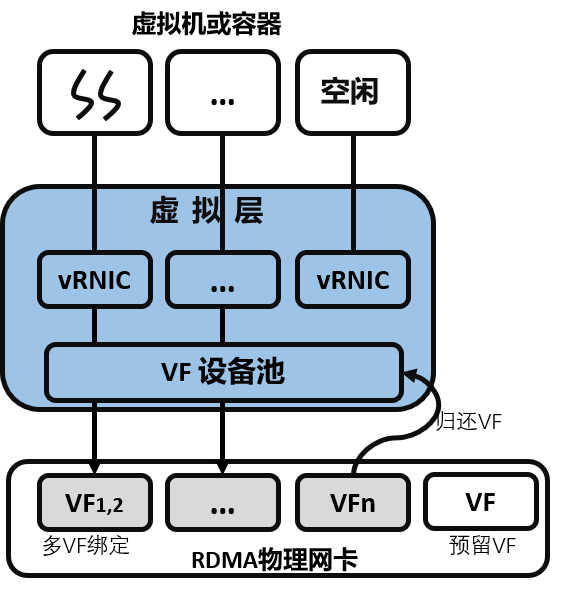
\includegraphics[width=0.9\linewidth]{images/vf-mapping}
	\caption{Management of vRNIC Mapping}
	\label{fig:vf-mapping}
\end{figure}

As Figure~\ref{fig:vf-mapping} shows: First, the virtual layer constructs a dynamic VF pool. The initial number of VFs in the pool is usually the number of pre-determined virtual instances. If lack of free VFs in the pool, the device pool can dynamically expand the number of VFs. Second, the virtual layer supports dynamic mapping between vRNIC and VF. When all virtual RDMA resources have been destroyed, the virtual layer marks the VF as idle and puts it back into the pool. So that the virtual layer can support the number of vRNICs that exceed the VF limit. Finally, the virtual layer supports various mapping relationships between vRNICs and VFs. For example, load balancing can be meted by map a vRNIC with multiple VFs. VF resources are saved by mapping multiple vRNICs of the same virtual instance to the single VF. 

For multiple containers and virtual machines, if shared memory files for vRNIC driver are not isolated, they can be discovered by every container through scanning files. In order to solve this problem, we run the virtual machine in a isolated container environment. As shown in in Figure~\ref{fig:interface-isolate}, based on the container's mount namespace~\cite{mount-ns}, we respectively place the shared files of each vRNIC in the dedicated directories and mounts each directory to the corresponding container(including containers running virtual machines). As a result, due to the isolation of the mount namespace, the shared files of each vRNIC in the virtualization layer are only visible to the used container or virtual machine.  

\begin{figure}[!ht]
	\centering
	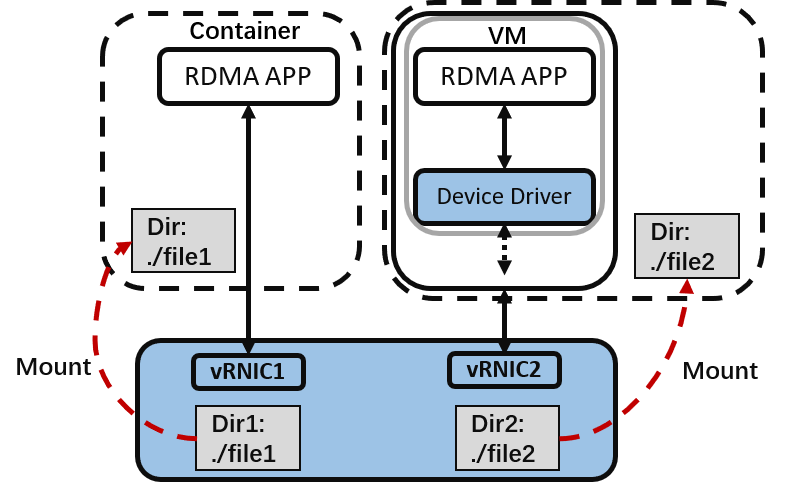
\includegraphics[width=1.0\linewidth]{images/interface-isolate}
	\caption{Isolation for vRNIC driver}
	\label{fig:interface-isolate}
\end{figure}

\subsection{Virtual RDMA Management}
To maintain portability and realize RDMA network management, RDMA connections between vRNICs cannot be established by the physical address of VFs. But this problem has a solution that uniRDMA virtual layer acts as a software RDMA switch or router for virtual RDMA network configuration and routing management, etc.

RNICs are usually managed by the subnet manager in the cluster. For the same purpose, a control center is set up in uniRDMA to assign virtual RDMA addresses vGIDs to each vRNIC and configure routing rules between vRNICs. As shown in Figure~\ref{fig:route-config} , the vRNICs are divided into two groups: group 1 and group 2; vRNICs in the same group are allowed to establish RDMA connections, and cross-group RDMA connections cannot succeed due to the isolated routing rules between group 1 and group 2.

\begin{figure}[!ht]
	\centering
	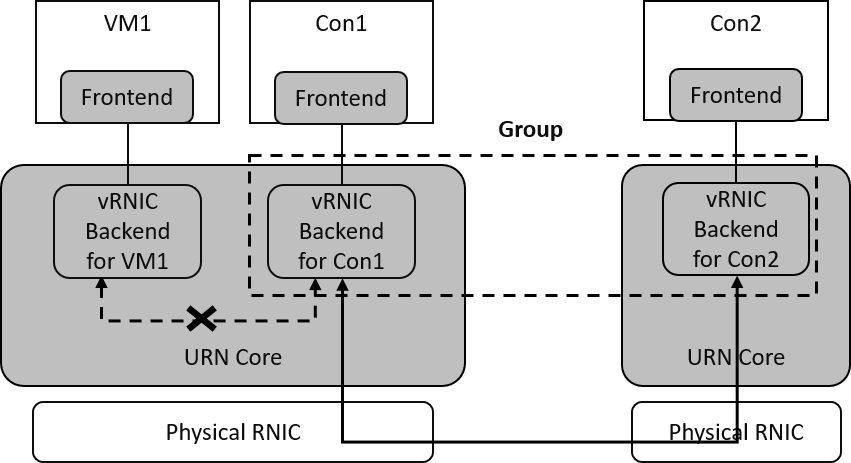
\includegraphics[width=1.0\linewidth]{images/route-config}
	\caption{Virtual RDMA Network Routing}
	\label{fig:route-config}
\end{figure}

Consistent with native RDMA, vRNICs in each virtual layer need to exchange each other's virtual RDMA addresses, virtual QP queue information, registered memory keys and other information to establish virtual RDMA connections. However, the vRNIC RDMA address is virtual, and does not recognized in RNIC. Therefore, the mapping relations between the virtual addresses of vRNICs and the physical addresses of VF needs to be exchanged between virtual layers. When establishing the virtual RDMA connection, the virtual RDMA address is converted to the physical address of the mapped VFs. Note that RDMA resources information, such as virtual QP number and memory keys, have been mapped to the VF interface by the map unit in vRNIC, they can all be recognized VF and directly used to create RDMA connection.

\subsection{Discussion}
Note that all vRNICs (including vRNICs' RDMA resources) are manipulated in the virtual layer. Thus, in virtual layer, there are avaliable for more managements. And we introduce some ongoing features for clouds:

Control police for clouds: To manage the resources precisely, there are lots of important polices in clouds, e.g. QoS, metering and so on. In uniRDMA, we can still meet these control features in virtual layer for these resons:  First,  the virtual layer can monitoring the QPs or CQs for RDMA traffic information, such as,  size and status of one RDMA work request, because all RDMA resources (including QPs and CQs) are mapped at host's virtual layer; Second, the virtual layer can  control the virtual RDMA traffic by controling the RDMA resources,  with the help of host RDMA libraries. For an example,  we can destroy the QP in the virtual layer when a RDMA connections' traffic is excessive.  These will cause more CPU overhead in the host virtual layer, but would not impact the performance of RDMA applications in clouds.

Virtual Instances Migration: Migration is important  for both containers and VMs in clouds with many benifits, e.g. resource utilization and fail-over. With the virtual RDMA network , uniRDMA can support offline migration without reconfiguring the physical RDMA network for applications. In specific,after rebooting the migrated virtual instance, the application can rebuild the RDMA connection  only by modifing the address mapping in software virtual layer. Currently, for live migrations, it is still hard because memory regions in RDMA application may be uncertain under bypassing or one-side communication. Thus, uniRDMA does not support live migrations for both VMs and containers.

Other network extensions: RDMA can also be exploited to optimize the performance of other network applications,  such as TCP/IP.  Existing works include vSocket ~\cite{wang2019vsocket}, SockDirect~\cite{li2019socksdirect} so on. In uniRDMA, we can extend the simiar design for socket applications in containers and VMs: unified vNICs and the driver of vNICs in containers or VMs.  The difference in the virtual layer is mainly how to emulate the vNICs based on host RDMA's libraries. 
\section{Implementation}
%我们在Linux环境中实现了\sys框架:
 We implement a prototype for \sys in Linux environments. The hypervisor of VM is QEMU/KVM and the container engine is Docker. The vRNIC frontend for VMs and containers is implemented differently. The \sys core (with vRNIC backends) includes about 2000 lines codes in the host user-space. And the management center is implemented through Zookeeper to the information for RDMA resources (such as RDMA address mapping, the numbers of VFs) and the policies (such as QP limit, QoS). In addition, we modified the Verbs library libibverbs-41mlnx1, the library about connection management librdma-cm, and the user-space RNIC driver libibverbs-41mlnx1. And we do some necessary work in host kernel, such as caching GPA into RNIC, mapping DoorBells. In this section, we introduce some representative implementation details:
 
 % 资源映射:根据资源所属于的物理地址空间,RDMA通信过程中主要有两类资源:内存资源(QP等),和设备资源(门铃).
 \subsection{Resource Mapping}
According the physical address space, there are mainly two kinds of resources for RDMA: memory resources (e.g. QPs, MRs) and device resources (e.g. DoorBells). 
 
 % 对于内存资源: 在虚拟机中, 我们利用vhost-user的半虚拟化技术构建vRNIC后端,vRNIC后端可以与虚拟机共享整块内存。 在具体操作中,需要先借助vRNIC前端将GVA转换为GPA;然后,在vRNIC后端中,由于vRNIC后端已经和虚拟机共享整块内存,因此,GPA可以被线性转换为HVA。但是,从GVA到GPA的转换由于guest OS的内存管理, 可能存在非线性的不连续现象,进一步导致vRNIC后端中映射的HVA区域也是不连续的。此时,在后端可以利用mremap系统调用重新映射虚拟内存,以将对应的物理页面映射到连续的HVA区间.
 For memory resources (e.g. QP), the mapping in VMs is as shown in Figure \ref{fig:qp-map}. We set the whole memory of the guest is shared in QEMU process, and the shared memory file path is registered in the vRNIC backend process. Because different processes can share the physical memory through the shared memory file. (1) The application in the guest allocate the QP buffer, and the buffer is using the shared memory in the host. The physical pages in the guest is pinned in the guest kernel. (2) The vRNIC backend receive the GPAs of the QP buffer. Note that the GPAs may not be contiguous. If we directly map the shared memory file through dis-contiguous GPAs (offsets), the obtained HVA also be dis-contiguous and cannot be used as the QP buffer. Thus, the vRNIC backend remap the corresponding shared memory to a new contiguous virtual memory region, and use it as the QP buffer.
 
 The mapping in containers is simple: The application in containers explicitly allocate the shared memory as the QP buffer in the modified Verbs libraries. Note that each QP, QP or MR uses a unique shared memory file. The vRNIC backend directly use the mapped region from the corresponding shared memory file.
\begin{figure}[!ht]
	\centering
	\includegraphics[width=1\linewidth]{images/qp-map.png}
	\caption{QP Mapping}
	\label{fig:qp-map}
\end{figure}

 

 For RDMA device resources (e.g. DoorBells), the mapping in VMs is as shown in  Figure \ref{fig:db-map}. (1) The application in the guest request the DB-HPA handle to the vRNIC backend. There are two reasons to do it: first, the page tables is different between the QEMU process (the guest) and the vRNIC backend processes, and the mapping from QEMU-HVA to DB-HPA must be done in QEMU process; second, the physical RDMA context is centrally maintained in the vRNIC backend, including the DB. (2) The application vRNIC backend receive the request and map the physical DoorBell. (3) The vRNIC backend obtain the DB-HPA handle through the helper module in the host kernel and return the handle to the application in the guest. (4) The vRNIC backend map a virtual DoorBell, forwards the GPA and DB-HPA handle to the helper module in the host kernel, and the helper module translate the GPA to QEMU-HVA. (5) The helper module remaps the QEMU-HVA to the DB-HPA. The helper module is implemented based on the para-virtrualization vhost modules, which provide high I/O performance  between the guest and the host kernel.
 
 In containers, the mapping of DoorBells is similar as the above. The only difference is that the application in the container directly forwards the virtual memory address to the helper module in the host kernel, through a simple costumed  character device driver. 
 \begin{figure}[!ht]
	\centering
	\includegraphics[width=1\linewidth]{images/db-map.png}
	\caption{DoorBells Mapping}
	\label{fig:db-map}
\end{figure}
 

\subsection{Register MR in the Host}
When vRNIC backend receives the registering MR commands and registers the MR, it should use the GVA as the virtual address when caching the page table for physical RNIC. And the physical RNIC can directly access the physical pages through the GVA in the work request of the application, instead of translating the GVA to the HVA in the data path. 

To implement it, we modified the OFED driver and the Verbs library in the host: the OFED driver can receive the GVA parameter when register MR, and fillwith the cached page table with the GVA as the virtual memory address.



\section{Evaluation} \label{eval}
In this section, we evaluate the performance of \sys based on the RDMA test tools and real applications. We expect to answer the following questions:

\begin{itemize}
\item How about the performance of \sys compared to that of native RDMA for both VMs and containers?
\item Can \sys be adapted to the real-world RDMA applications in both VMs or containers?
\end{itemize}

\subsection{Experiment Methodology}
All experiments are carried out on two servers. The settings mainly include three parts: host server, container and virtual machine. 

Each host server is equipped with 4 Intel Xeon E7-4850 2.40GHz 16-core CPUs and 1 TB RAM. The RNIC used is Mellanox ConnectX-3 56 Gb/sec, which performs RDMA communication under Infiniband.  The operating system is CentOS 7.4.1708 (Linux 3.10.0-693.el7.x86\_64). The RDMA driver installed on the host server is Mellanox OFED 4.4-2.0.7.0~\cite{mlnx-ofed}. To keep the consistence, VMs and containers are built based on the same OS images as host. All virtual machines are based on QEMU(5.1.50)~\cite{qemu} enabled with KVM~\cite{kvm}. We provide 16 cores and 64 GB memory for each VM. We run containers using Docker(18.06.1-ce)~\cite{docker} and limit the CPU and memory resources to the same settings as the VM. In addition, all the applications are compiled with GCC/G++ 4.8.5 with the O3 compilation configuration. 


\subsection{Basic benchmark}
Throughput and latency are the key target of network performance. RDMA supports two different data transmission modes: one-sided and two-sided. Due to the difference performance between them, we evaluate them respectively.

Based on the RDMA benchmark test tool perftest~\cite{perftest}, we evaluated the throughput and latency of \sys, native RDMA, hardware virtualization SR-IOV, and software virtualization FreeFlow in virtual machines or containers. For two-sided operations (Send and Recv), we use the ``ib\_send\_bw'' and ``ib\_send\_lat'' commands; for one-sided operations (Write and Read), with Write as the representative, we use the ``ib\_write\_bw'' and ``ib\_write\_lat'' commands. The specific process is: after the RDMA connection is established between the client and the server, the bytes of transmitted message each time will be increased from 4B to 1MB, the data will be iteratively transmitted 1000 times with each message size, and finally the average throughput and latency are calculated.

(1) Throughput: The results of two-sided operation are shown in Figure~\ref{fig:send-bw}, and the one of one-sided operation are shown in Figure~\ref{fig:write-bw}. Whether \sys is in a virtual machine or in a container scenario, the throughput of its two-sided and one-sided operations is similar as SR-IOV and close to native RDMA.

Compared with FreeFlow, when the message is small, the throughput of \sys has reached 4-6 times that of FreeFlow. Because FreeFlow forwards all data commands to the software virtualization layer for processing. Therefore, the forward latency gradually accumulates and decrease the throughput significantly. However, \sys maps all RDMA resources to execute data commands in the user space of the container or virtual machine. Therefore, there is no latency for commands forwarding in data path.

\begin{figure}[!ht]
	\centering
	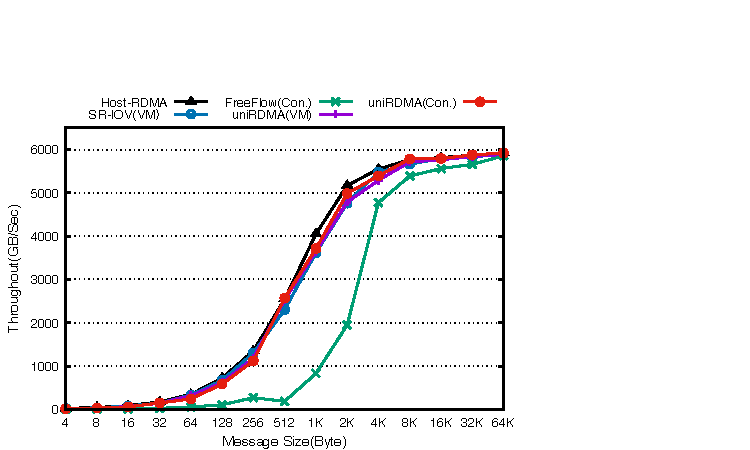
\includegraphics[width=1.0\linewidth]{images/send-bw.pdf}
	\caption{The Throughout of RDMA Send and Recv}
	\label{fig:send-bw}
\end{figure}

\begin{figure}[!ht]
	\centering
	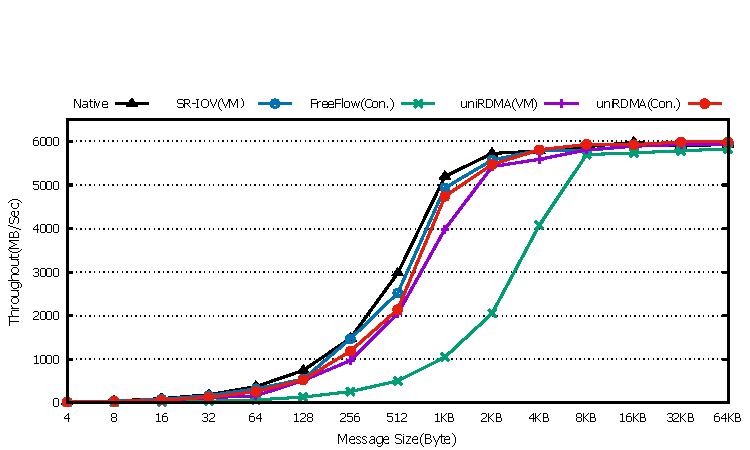
\includegraphics[width=1.0\linewidth]{images/write-bw.pdf}
	\caption{The Throughout of RDMA Write}
	\label{fig:write-bw}
\end{figure}

When the message gradually increases, such as reaching 64KB, the throughput of each framework tends to be consistent. The reason is that the bandwidth is saturated, and the delay overhead of FreeFlow has been covered by waiting delay in RNIC.

(2) Latency: The results of two-sided operation are shown in Figure~\ref{fig:send-lat}, and the one of one-sided operation are shown in Figure~\ref{fig:write-lat}. Whether \sys is in a virtual machine or in a container scenario, the latency of its two-sided and one-sided operations is similar as SR-IOV and close to native RDMA.

Compared with FreeFlow, when the message is small, the latency of \sys has reached 40\%~60\% of FreeFlow because of FreeFlow's forwarding latency. Also, when the message gradually increases, such as reaching 64KB, the latency of each framework tends to be consistent. Because the main latency has been caused by RNIC data processing.

\begin{figure}[!ht]
	\centering
	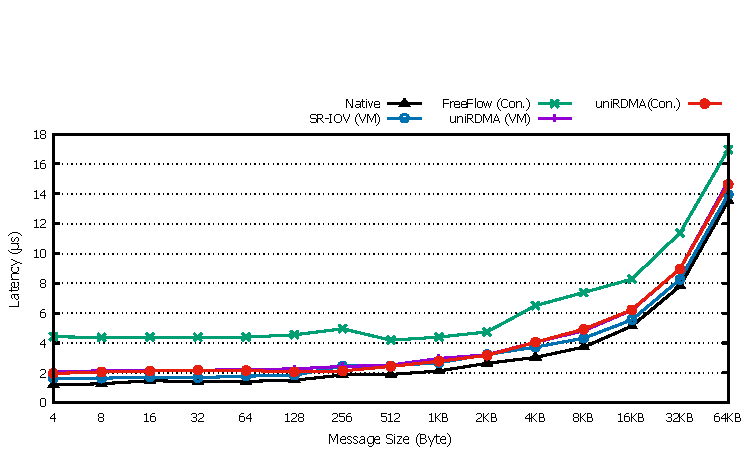
\includegraphics[width=1.0\linewidth]{images/send-lat.pdf}
	\caption{The Latency of RDMA Send and Recv}
	\label{fig:send-lat}
\end{figure}

\begin{figure}[!ht]
	\centering
	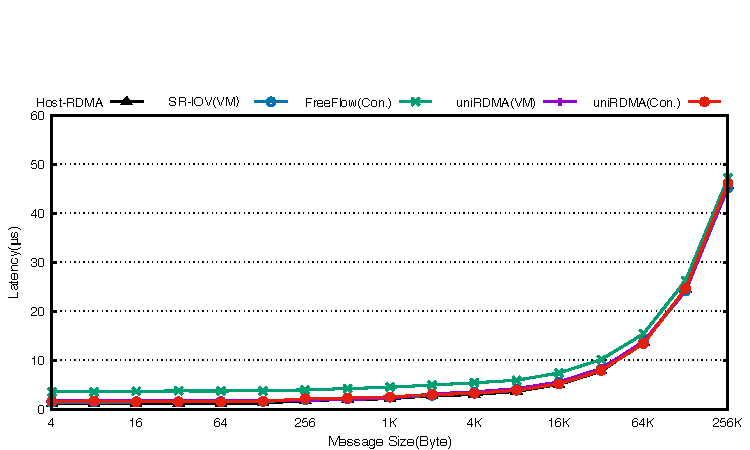
\includegraphics[width=1.0\linewidth]{images/write-lat.pdf}
	\caption{The Latencty of RDMA Write}
	\label{fig:write-lat}
\end{figure}

\subsection{Real-world Applications}

The worth of RDMA is mainly about its optimized performance in real-world applications. RDMA virtualization needs to maintain the performance close to native RDMA. Therefore, we evaluate \sys and other frameworks in high-performance computing benchmark Graph-500. Graph-500 is a benchmark framework used to test the performance of the Message Passing Interface (MPI). Based on the constructed graph structure, users test the performance of breadth-first search (BFS) and single source shortest path (SSSP). The performance index is the number of edges traversed per second (traversed edges). per second, TEPS), the larger the value, the better the performance.

In this paper, the node scale of the computational graph in Graph-500 is set to 26, and the ratio of edges to points is set to the default parameter of 16. The constructed graph has a total of 2$^{25}$ vertices, with 2$^{29}$ edges, the entire graph occupies approximately around 16GB. When testing BFS and SSP, 16 MPI processes are scattered and executed on two nodes in turn, and the average value is taken according to the results of 12 tests. The data obtained is shown in Table Figure~\ref{fig:graph-500} (because there are core dump problems when using FreeFlow for Graph-500, the corresponding data is lacking).

As shown in Figure~\ref{fig:graph-500},  the performance of \sys is close to native RDMA. Because \sys bypasses the kernel and virtualization layer in the data path, and there is no forwarding latency.

\begin{figure}[!ht]
	\centering
	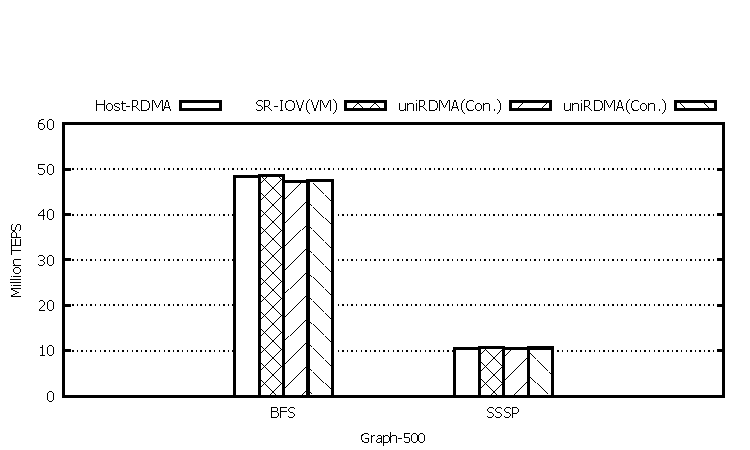
\includegraphics[width=1.0\linewidth]{images/graph-500.pdf}
	\caption{The Performance of Graph-500}
	\label{fig:graph-500}
\end{figure}
\section{Related Work} \label{relatedwork}

\textbf{Traditional TCP/IP:}\qquad TCP/IP is the basic network for each tenant in data centers. Several software solutions were proposed for traditional network virtualization. For both VMs and containers, virtual network interface cards (vRNICs) are one solution, e.g. virtio-net~\cite{virtio-russell2008}, vhost-net~\cite{vhost-net},  vhost-user-net~\cite{vhost-user-net} for VMs and veth~\cite{veth} for containers. These vRNICs are implemented in VM's or container's different space (i.e. kernel space and user space). Software-based switch, also knowed as virtual switch, in the local host brides the vNIC to physical NIC. Virtual switch can run in user space (e.g. Snabb Switch~\cite{snabb}), kernel space(e.g. Linux bridge~\cite{linux-bridge}), or both(e.g. Open vSwitch~\cite{ovs-2015}). 

\textbf{Hardware-based RDMA virtualization:}\qquad SR-IOV~\cite{sr-iov} splits a physical PCI-e device to multiple PCI-e devices, which can be allocated to VMs, providing near-native performance. In comparison to software-baed virtualization, it lacks of refficient resource management and suffers from the flexibility issue due to its virtual layer is realized in hardware. In uniRDMA, the isolation of SR-IOV are utilized and the unscalable problems are solved by dynamic vRNIC mapping. 

\textbf{Software-based RDMA virtualization:}\qquad FreeFlow~\cite{kim2019freeflow} forwards all RDMA commands from containers to the FreeFlow router (FFR) including data path. It intercepts the commands between applications and NIC drivers such as creating QP/CQ and sending/receiving data. The key different between FreeFlow and uniRDMA is that FreeFlow does capture data path commands to fitting in the container environment. Its data path commands, which accounts for the majority compared to the control path, costs extra forward latency. HyV~\cite{pfefferle2015hybrid} and MasQ~\cite{he2020masq} are designed for VMs. They achieve zero-copy and by-pass by mapping all resources. However, the implementation of memory mapping are different that is uniRDMA maps memory between virtual layer and VM's application. Moreover, HyV/MasQ backend is in kernel space while uniRDMA backend is in user space for more manageability and lightweight.

\section{Conclusion}
In this paper, we design a unified RDMA virtualization framework, namely uniRDMA, which consists of single user-space virtual layer and general uniVerbs interfaces. In the user space virtual layer: the isolated and high-performance vRNICs are virtualized based on the VFs from SR-IOV; In the uniVerbs interfaces: uniRDMA uses shared files to realize general I/O channel for VMs and containers; the isolation of interface is ensured with mount namespace in containers; uniVebrs realizes zero-copy and bypassing virtual layer in RDMA data path, by mapping all RDMA resource between vRNIC and RDMA applications. The experimental results show that uniRDMA has high performance close to native RDMA while meeting generality and management.





%%
%% The next two lines define the bibliography style to be used, and
%% the bibliography file.
\bibliographystyle{ACM-Reference-Format}
\bibliography{reference}

%%
%% If your work has an appendix, this is the place to put it.
%\appendix



\end{document}
\endinput
%%
%% End of file `sample-sigconf.tex'.
